% ----------------------------------------------------------
% The RI5cy Study Case
% ----------------------------------------------------------
\chapter{The RI5CY Case Study}
\label{chapter:ri5cy}

The algorithm to generate Pipeline Properties, proposed in Chap.~\ref{chapter:algorithm},  was evaluated with a case study for the RI5CY processor core. RI5CY is a 4-stage pipeline processor core based on the RISC-V architecture. Its implementation is open-source and powered by PULP Platform \cite{pulp}.

For this case study, a \textit{SystemC-PPA-compliant} \cite{paper-pdd} model for the chosen core was implemented as a sequential CPU model. The properties were then automatically generated using DeSCAM \cite{descam}. From these automatically generated properties, the Pipeline Properties were finally created using the merging Pipeline Algorithm. 

This chapter starts with a brief discussion about the RISC-V Implementation Set Architecture and the RI5CY processor core in Sec.~\ref{section:ri5cy_core}. Next, the ESL implementation compliant to the SystemC-PPA specification is detailed in Sec.~\ref{section:ri5cy-systemc-ppa}. Then, the DeSCAM generated properties and the Pipeline Properties are presented and explained in Sec.~\ref{section:ri5cy_pipe_ppt}. Finally the \SSQED{} Properties are presented in Sec.~\ref{section:ri5cy-s2qed-ppt}.

\section{The RI5CY Processor Core}
\label{section:ri5cy_core}

\textit{Instruction Set Architecture}~(ISA), is the set of instructions that a computer, or more specifically a processor core, can execute. Some of the specification provided by the ISA are which operations the processor can perform, how the memory is addressed and the type and size of the instruction operands \cite{book-comp-arch}.

A \textit{Reduced Instruction Set Computer}~(RISC) is a computer that has a small set of instructions. These instructions have a simple fixed length encoding, and they take similar number of \textit{clock} cycles to execute \cite{book-comp-arch}. Some examples of RISC architectures are AMRv7, MIPS and RISC-V.

RISC-V is an open ISA that offers both a small base integer ISA that can be used by itself, and optional standard extensions. As an open and free to use architecture, it was initially intended to support computer architecture research and education \cite{spec-riscv}. Even so, its popularity increased rapidly and there are open-source simulators, compilers, debuggers and implementations in HDL for RISC-V available \cite{book-comp-org}. One of these open-source implementations is the RI5CY processor powered by PULP Platform \cite{pulp}. This implementation is used as case study in the present work and some important details are presented in this section. 

RI5CY is an in-order \textit{32 bits} core and has a pipeline with 4 stages. Besides the support for the \textit{RV32I} Base Integer Instruction Set, it has also support for the \textit{RV32C} Standard Extension for Compressed Instructions and \textit{RV32M} Integer Multiplication and Division Instruction Set Extension, and optional support for \textit{RV32F} Single Precision Floating Point Extensions. This core also implements the following PUPL specific extensions:  Post-Incrementing load and stores, Multiply-Accumulate extensions, ALU extensions, and Hardware Loops.

However, this case study is focused on the \textit{32bits} Integer Base Instructions set \SSSAY{[maybe some standard extensions if time allows it]} as detailed in Sec.~\ref{section:ri5cy-systemc-ppa} of this chapter. Before that, however, some aspects of the pipeline, memory protocol and Load-Store Unit of the RI5CY core are briefely discussed. These implementation aspects are important for the understanding of the ESL model and for the property generation as well.

For detailed information about all the RI5CY extensions, the reader may refer to the RI5CY User Manual \cite{manual-ri5cy}.

\subsection*{RI5CY Pipeline}

The RI5CY core implements a 4-stage pipeline: instruction fetch (\textit{IF}), instruction decode (\textit{ID}), execute (\textit{EX}) and write-back (\textit{WB}). However, most of the instructions in the base integer set, like arithmetic and logic operations, uses only the first three stages. The \textit{WB} stage is used, for example, when loading data from the data memory. Fig.~\ref{fig:ri5cy_pipeline} depicts the pipeline structure and its main signals.

\begin{figure}[htb!]
	\centering
	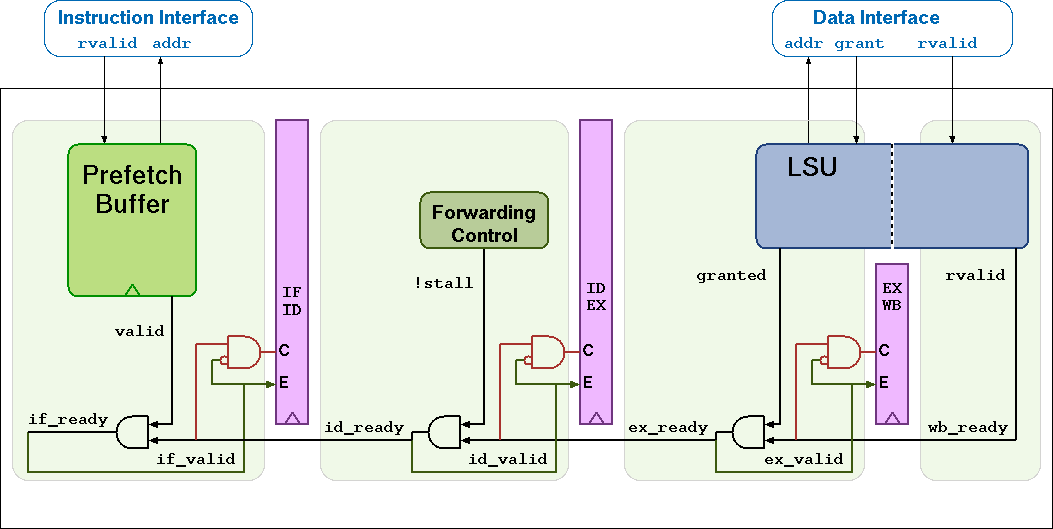
\includegraphics[width=\textwidth]{images/ri5cy_pipeline.png}
	\caption{RI5CY pipeline diagram \cite{manual-ri5cy}.}
	\label{fig:ri5cy_pipeline}
\end{figure}

The \textit{ready} signal of each stage propagates from right to left and are used to inform the previous stage that the current stage is ready to operate. In this sense, each stage can finish its execution independently from the previous, but they cannot propagate if the next one is not ready, the pipeline \textit{stalls}. 

\subsection*{RI5CY Load-Store Unit}

\textit{The Load-Store Unit}~(LSU) is the component of the core responsible to access the data memory. As shown in Fig.~\ref{fig:ri5cy_pipeline}, the LSU belongs to two pipeline stages: \textit{EX} and \textit{WB}. It means that a request to the data memory is sent already in the \textit{EX} stage. To illustrate this behaviour better, consider a \textit{LOAD} instruction in the \textit{ID} stage. In the next \textit{clock} cycle, the access address is computed in the \textit{EX} stage, and the LSU sends a request to the data memory in the same cycle. When the data arrives from memory, the LSU will write it to the correspondent register in the \textit{WB} stage. The memory access protocol is detailed next.

\subsection*{RI5CY Memory Access Protocol}

In order to access the data memory, the LSU sets the output address with the right address and sends a request signal. The LSU waits for a grant signal from the memory that can come in the same \textit{clock} cycle as the request or any number of \textit{clock} cycles later. After receiving the grant signal, the LSU can optionally change the outputs and make a new request or just set the request signal to \textit{low}. If it was a read from memory request, e.g. \textit{LOAD} instruction, the memory will send the data along with a valid signal one or more \textit{clock} cycles after the grant signal. All the LSU signals can be found in Table~\ref{tab:lsu-signals} with a brief description. 

\begin{table*}[htb!] 
	\centering 
	\caption{LSU port signals of RI5CY processor\cite{manual-ri5cy}.} 
	\label{tab:lsu-signals}
	\begin{tabular}{l|c|p{7cm}} 
		\multicolumn{1}{c}{\bfseries Signal} & \multicolumn{1}{c}{\bfseries Port Direction} & \multicolumn{1}{c}{\bfseries Description} \\     
		\hline	
		$data\_req\_o$  &  output & Request ready, must stay high until $data\_gnt\_i$ is        high for one cycle \\
		\hline
		$data\_addr\_o$[31:0]  &  output & Address \\
		\hline
		$data\_we\_o$  &  output & Write Enable, high for writes, low for reads. Sent            together with $data\_req\_o$ \\
		\hline
		$data\_wdata\_o$[31:0]  &  output & Data to be written to memory, sent together with     $data\_req\_o$ \\
		\hline
		$data\_rdata\_i$[31:0]  &  input & Data read from memory \\
		\hline
		$data\_rvalid\_i$  &  input & $data\_rdata\_i$ holds valid data when                     $data\_rvalid\_i$ is high. This signal will be high for exactly one cycle per        request. \\
		\hline
		$data\_gnt\_i$  &  input & The other side accepted the request. $data\_addr\_o$ may     change in the next cycle \\
		\hline
	\end{tabular} 
\end{table*}

The instruction memory access performed by the instruction fetcher of the core is similar to the data memory protocol. The only difference is that the instruction fetcher does not have any \textit{write} interface, since the instruction memory is only read by the core. The instruction fetcher signals are presented in Table~\ref{tab:imem-signals}.

\begin{table*}[htb!] 
	\centering 
	\caption{Instruction memory port signals of RI5CY processor \cite{manual-ri5cy}.} 
	\label{tab:imem-signals}
	\begin{tabular}{l|c|p{7cm}} 
		\multicolumn{1}{c}{\bfseries Signal} & \multicolumn{1}{c}{\bfseries Port Direction} & \multicolumn{1}{c}{\bfseries Description} \\     
		\hline	
		$instr\_req\_o$  &  output & Request ready, must stay high until $instr\_gnt\_i$ is high for one cycle \\
		\hline
		$instr\_addr\_o$[31:0]  &  output & Address \\
		\hline
		$instr\_rdata\_i$[31:0]  &  input & Data read from memory \\
		\hline
		$instr\_rvalid\_i$  &  input & $instr\_rdata\_i$ holds valid data when $instr\_rvalid\_i$ is high. This signal will be high for exactly one cycle per request. \\
		\hline
		$instr\_gnt\_i$  &  input & The other side accepted the request. $instr\_addr\_o$ may change in the next cycle \\
		\hline
	\end{tabular} 
\end{table*}

\section{SystemC-PPA Implementation}
\label{section:ri5cy-systemc-ppa}

For this case study, an ESL model was implemented to comply with the RI5CY core implementation. The core user manual along with the existent RTL implementation were used to extract the specifications for the system-level. Therefore, the PDD flow is not followed to implement the RTL design, as it already exists. The goal was to create a SystemC-PPA compliant model of a processor based on the RISC-V architecture such that the generated set of properties would hold to its RTL implementation.

The proposed ESL model does not comprise the RI5CY extensions and implements only a restrict set of instructions from the \textit{RV32I} Base Integer Instruction set of the RISC-V ISA. They are the arithmetic and logic instructions, \textit{load} and \textit{store} instructions, \textit{branch} and \textit{jump} instructions, and \textit{LUI} and \textit{AUIPC}.

The block diagram in Fig.~\ref{fig:sim-ri5cy-diagram} shows the configuration implemented for simulating the ESL model of the core. The Register File and the Memory modules were imported from the RISC-V example in the \textit{DeSCAM} repository \cite{descam}. The Register File has 32 registers where register 0 is \textit{read-only}, and the Memory module implements a memory for both instruction and data. For this reason, a memory interface had to be implemented in order to parse memory requests from the core, as it has separate ports for instructions and data.

\begin{figure}[htb!]
	\centering
	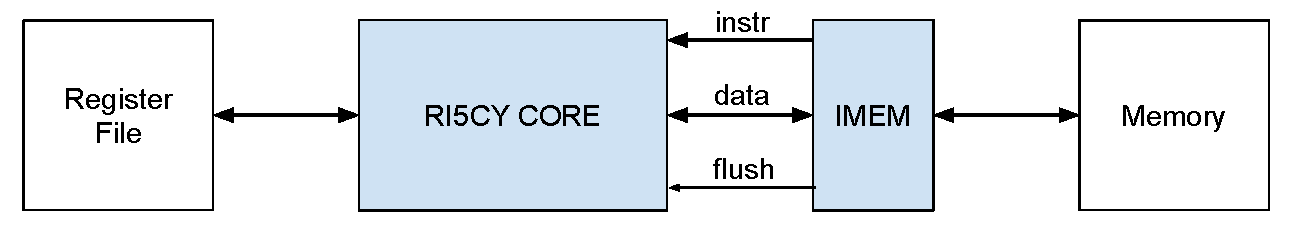
\includegraphics[width=\textwidth]{images/sim-block-diagram.pdf}
	\caption{Block diagram of the system-level implemented for the RI5CY core.}
	\label{fig:sim-ri5cy-diagram}
\end{figure}

As shown in the block diagram of Fig.~\ref{fig:sim-ri5cy-diagram}, the RI5CY CORE has four \textit{I/O} interfaces. Two for memory transactions, instruction and data, one for communicating with the Register File and a \textit{flush input} signal. Their declaration can be seen in the code snippet in Fig.~\ref{fig:ri5cy-sc-module} that shows the class declaration of the SystemC module of the processor core.

\begin{figure}[htb!]
    \begin{lstlisting}[language=c++]
    class ISA_ri5cy : public sc_module {
    public:
        //Constructor
        SC_HAS_PROCESS(ISA_ri5cy);
        ISA_ri5cy(sc_module_name name) {
        SC_TH   READ(run);
        }
        //ports for communication with instr mem
        master_in<unsigned int> instr_in;
        master_out<unsigned int> instr_req;
        
        //ports for communication with data mem
        master_in<unsigned int> data_in;
        blocking_out<CUtoME_IF> data_out;
        
        // ports for communication with register file
        shared_in<RegfileType> fromRegsPort;
        master_out<RegfileWriteType> toRegsPort;
        
        // flushing signal for RTL (always false for ESL simulation)
        shared_in<bool> flush_in;
        
        enum Sections {FETCH_PH, DECODE_PH, EXECUTE_PH};
        // [...] variables and helping functions
        void run(); // fsm
    };\end{lstlisting}
    \caption{SystemC class of the RI5CY core.}
    \label{fig:ri5cy-sc-module}
\end{figure}

The instruction memory interface is of type \textit{Master}, and it has two signals. One \textit{output} signal to send the request address, and an \textit{input} signal that receives the requested instruction. The \textit{Master} interface is \textit{non-blocking} and simplifies the instruction memory protocol. Therefore, no wait signal is created for this interface. This is possible because each property will have a triggering condition that an instruction of a specific type is fetched. Thus, no waiting upon the instruction memory is needed.

On the other hand, the data memory interface has a \textit{blocking output} port for making the requests, and a \textit{Master input} port to read the data. This means that the processor must wait for a synchronization signal from the data memory upon a request. If the request is a \textit{read} operation, the incoming data is available after synchronization. For this reason, the \textit{input} port is \textit{non-blocking} of type \textit{Master}.

The interface for communicating with the Register file is also \textit{non-blocking}. In fact, the register file is modeled as an external module at the system-level, however it is embedded to the core in the RTL implementation. This modeling decision illustrates that the RTL implementation choices are not constrained by the system-level model. In this case, during the \textit{refine-and-implement} phase of the PDD flow, the designer would have simply to match the ESL ports to the internal signals of the RTL. Since the register can be read as an internal variable, the type of interface employed was the \textit{Shared} interface for \textit{input} and \textit{Master} for \textit{output}, both are \textit{non-blocking} interfaces.

The \textit{flush} signal is part of the enriched SystemC-PPA, and it is included in the model to reflect the flushing behaviour of the pipeline. Execution of some instructions may cause the pipeline to flush, e.g. when a branch instruction is evaluated and the branch is taken, the consecutive instruction, already fetched and executing in the pipeline, must be flushed. This behaviour is not modeled by the ESL because its execution is sequential, and an instruction only starts executing after the previous one is concluded. Therefore, there is no need for \textit{flushing}. The inclusion of the \textit{flush} signal at the ESL should not change its behaviour during simulation, but it will change the generated property set. The properties will have one operation for when the \textit{flush} signal is asserted and one for when it is not. The designer will then refine the flush macro into the corresponding implemented signal, e.g. the branch decision signal. 

The IMEM module is a memory interface that parses the separated instruction and data memory requests into a request to the single port of the memory model. It also feeds the core with a \textit{flush} signal always set to false, so it does not interfere in the simulation. This module, like the Register File and the Memory model, is only used for simulating the RI5CY core. The only module that is interpreted by \textit{DeSCAM} to generate the property set is the core module, which is the DUV.

An outline of the \textit{run()} function is shown in Fig.~\ref{fig:ri5cy-run-outline}. This function implements the main behaviour of the core. It runs infinitely and is divided into three sections, \textit{FETCH\_PH}, \textit{DECODE\_PH} and \textit{EXECUTE\_PH}. These three phases directly relate to the pipeline stages of the processor. However, the write back stage is not explicitly shown. This is because this \textit{WB} stage is only used by the LSU, and its important state is created as a result of the memory \textit{blocking} interface. 

\begin{figure}[htb!]
    \begin{lstlisting}[language=c++]
    void ISA_ri5cy::run() {
        nextsection = Sections::FETCH_PH;
        while (true){
            if (section == Sections::FETCH_PH){
            //[...]
            nextsection = Sections::DECODE_PH;
            } else if (section == Sections::DECODE_PH){
            //[...]
            nextsection = Sections::EXECUTE_PH;
            } else if (section == Sections::EXECUTE_PH) {
                if(getInstrType(encodedInstr) != InstrType::INSTR_UNKNOWN){
                    if (getEncType(encodedInstr) == ENC_R){...}
                    else if (getEncType(encodedInstr) == ENC_I_I){...}
                    else if (getEncType(encodedInstr) == ENC_I_L) {...}
                    else if (getEncType(encodedInstr) == ENC_S) {...} 
                    else if (getEncType(encodedInstr) == ENC_B) {...} 
                    else if (getEncType(encodedInstr) == ENC_U) {...} 
                    else if (getEncType(encodedInstr) == ENC_J) {...} 
                    else if (getEncType(encodedInstr) == ENC_I_J) {...}
            }
            nextsection = Sections::FETCH_PH;
    }}}\end{lstlisting}
    \caption{Code outline from the \textit{run()} function of RI5CY core.}
    \label{fig:ri5cy-run-outline}
\end{figure}

\subsection*{The FETCH\_PH section}

This section is depicted in Fig.~\ref{fig:ri5cy-fetch-ph} and it simply fetches a new instruction. The variable \textit{fromReset} is only asserted in the first time this loop is executed. It is used to implement the \textit{reset} behaviour where the first request to the instruction memory is done. For the remaining execution, the instruction requests are done at the decode phase.

\begin{figure}[htb!]
    \begin{lstlisting}[language=c++]
    if (section == Sections::FETCH_PH){
        if(fromReset){
            instr_req->master_write(iaddr);
            pcIf = 0;
        }
        insert_state("IF");
        instr_in->master_read(encodedInstr);
        nextsection = Sections::DECODE_PH;
    }\end{lstlisting}
    \caption{FETCH\_PH section from the \textit{run()} function of RI5CY core.}
    \label{fig:ri5cy-fetch-ph}
\end{figure}

\subsection*{The DECODE\_PH section}

This section is shown in the code snippet of Fig.~\ref{fig:ri5cy-decode-ph}. The main attributions of this phase are updating the instruction fetching address, sending a new request to the instruction memory, and reading the register file. 

\begin{figure}[htb!]
    \begin{lstlisting}[language=c++]
    else if (section == Sections::DECODE_PH){
        flush_in->get(flush);
        if (flush) {
            iaddr = pcIf - 4 + getImmediate(prevInstr);
            instr_req->master_write(iaddr);
            prevInstr = encodedInstr;
            nextsection = Sections::FETCH_PH;
        } else {
            if(getEncType(encodedInstr) == ENC_J) {
            iaddr = pcIf + getImmediate(encodedInstr);
            instr_req->master_write(iaddr);
            insert_state("ID_J");
        } else if (getEncType(encodedInstr) == ENC_I_J) {
            fromRegsPort->get(regfile); //Read register contents
            iaddr = readRegfile(getRs1Addr(encodedInstr), regfile) + getImmediate(encodedInstr);
            iaddr = iaddr & 0xFFFFFFFE;
            instr_req->master_write(iaddr);
            insert_state("ID_I_J");
        } else {
            iaddr = iaddr + 4;
            instr_req->master_write(iaddr);
            insert_state("ID");
        }
        fromRegsPort->get(regfile); //Read register contents
        nextsection = Sections::EXECUTE_PH;
    }}\end{lstlisting}
    \caption{DECODE\_PH section from the \textit{run()} function of RI5CY core.}
    \label{fig:ri5cy-decode-ph}
\end{figure}

For the RI5CY core, the fetching address is not normally computed based on the PC, it is computed by incrementing the previous fetched address. The PC is used for instructions such as \textit{branch} and \textit{jumps} that need the address of the current executing instruction. The \textit{jump} instructions are executed already at the decode phase. Then, if the fetched instruction is a \textit{jump}, the new instruction address computation and the request to this address are done already in this section. The type \textit{ENC\_J} represents the instruction \textit{jal}, where the jumping address, i.e. the address of the next instruction to be fetched, is computed by adding the PC to the immediate field. The \textit{ENC\_I\_J} corresponds to the \textit{jalr} instruction. In this case, a reading to the register file is needed as the jumping address is computed by adding the register read value to the immediate field. The last bit of the resulting address is then masked to 0 and the new instruction is requested. The masking is done to comply with the behaviour specified by the RTL implementation. 

The \textit{flush} signal is also checked in the decode phase. The code inside the flush condition reflects the behaviour of the RTL if a \textit{flushing} is performed, and it determines how the properties for the \textit{flushing} cases are generated. In practice, this code is never executed during ESL simulation as the \textit{flush} signal always false. If a flush in the pipeline is required, a new instruction is fetched and its address is computed based on the PC and immediate field of the previously decoded instruction, which is currently in the \textit{EX} stage. 

\subsection*{The EXECUTE\_PH section}

As shown in Fig.~\ref{fig:ri5cy-run-outline}, the execute phase has a series of \textit{if} conditions and it will execute differently for each type of instruction. These types are based on the encoding types of the RISC-V ISA \cite{spec-riscv}.

The code snippet in Fig.~\ref{fig:ri5cy-enc-r} shows the execution phase to instructions for the \textit{ENC\_R} type. This type includes the register-register arithmetic and logic instructions. They are: \textit{add}, \textit{sub}, \textit{sll}, \textit{slt}, \textit{sltu}, \textit{xor}, \textit{srl}, \textit{sra}, \textit{or} and \textit{and}. The encoding and description of all instructions can be found in \cite{spec-riscv}. 

\begin{figure}[htb!]
    \begin{lstlisting}[language=c++]
    if (getEncType(encodedInstr) == ENC_R){
        aluOp1 = readRegfile(getRs1Addr(encodedInstr), regfile);
        aluOp2 = readRegfile(getRs2Addr(encodedInstr), regfile);
        aluResult = getALUres(getALUfunc(getInstrType(encodedInstr)), aluOp1, aluOp2);
        
        regfileWrite.dst = getRdAddr(encodedInstr);
        regfileWrite.dstData = aluResult;
        toRegsPort->master_write(regfileWrite); //WB
        
        pcIf = iaddr;
    }\end{lstlisting}
    \caption{Code for execution of instructions of \textit{ENC\_R} type from the \textit{run()} function of RI5CY core.}
    \label{fig:ri5cy-enc-r}
\end{figure}

During the execute phase, the \textit{ENC\_R} instructions read the values of the operands and compute the result from the ALU according to the operation of the instruction. The signals for writing the result values back to the register file are already set at the execute phase. For this reason, there is no \textit{WB} phase for those instructions. The arithmetic and logic instructions that operate with an immediate (I-type) are named as \textit{ENC\_I\_I} and have an execute phase very similar to the \textit{ENC\_R} instructions. The \textit{ENC\_I\_I} type comprises the instructions: \textit{addi}, \textit{slti}, \textit{sltiu}, \textit{xori}, \textit{ori}, \textit{andi}, \textit{slli}, \textit{srli}, and \textit{srai}. In the same way, the \textit{lui} and \textit{auipc} (U-type) instructions, called \textit{ENC\_U}, also execute in a very similar manner as the \textit{ENC\_R} type. The complete code can be found in \cite{descam}.

The listing in Fig.~\ref{fig:ri5cy-enc-i-l} shows the execution phase for the \textit{ENC\_I\_L} type that include the instructions \textit{lb}, \textit{lh}, \textit{lw}, \textit{lbu}, and \textit{lhu}. First, the access address is computed and used to send a request to the data memory. When the write operation is called on the \textit{blocking} port, a new important state is created. This new state corresponds to the \textit{WB} stage, and the write back signals to the register file are set at this point. The \textit{ENC\_S} type that comprises the \textit{sb}, \textit{sh}, and \textit{sw} instructions, have a similar execution phase, but it does not write back to the register file. 

\begin{figure}[htb!]
    \begin{lstlisting}[language=c++]
    else if (getEncType(encodedInstr) == ENC_I_L) {
        aluOp1 = readRegfile(getRs1Addr(encodedInstr), regfile);
        aluOp2 = getImmediate(encodedInstr);
        aluResult = getALUresult(ALU_ADD, aluOp1, aluOp2);
        
        pcIf = iaddr;
        
        //prepare memory access
        memoryAccess.req = ME_RD;
        memoryAccess.mask = getMemoryMask(getInstrType(encodedInstr));
        memoryAccess.addrIn = aluResult;
        memoryAccess.dataIn = 0;
        // Request load
        data_out->write(memoryAccess, "LOAD");
        
        // Load done
        data_in->master_read(fromMemoryData);
        
        regfileWrite.dst = getRdAddr(encodedInstr);
        regfileWrite.dstData = fromMemoryData;
        toRegsPort->master_write(regfileWrite); //WB
    }\end{lstlisting}
    \caption{Code for execution of instructions of \textit{ENC\_I\_L} type from the \textit{run()} function of RI5CY core.}
    \label{fig:ri5cy-enc-i-l}
\end{figure}

The branching instructions \textit{beq}, \textit{bne}, \textit{blt}, \textit{bge}, \textit{bltu}, and \textit{bgeu} are part of the \textit{ENC\_B} type, which execute phase is presented in Fig.~\ref{fig:ri5cy-enc-b}. The operands read from the register file are used to compute the branch decision, which determines if the branch will be taken or not. If the branch is taken, the instruction address is computed using the PC and the immediate field. At this point the PC holds the value of the current executing instruction. A new state must be inserted (line 11) because the PC is updated with the new instruction fetch address only on the next \textit{clock} cycle if the branch is taken.

\begin{figure}[htb!]
    \begin{lstlisting}[language=c++]
    else if (getEncType(encodedInstr) == ENC_B) {
        aluOp1 = readRegfile(getRs1Addr(encodedInstr), regfile);
        aluOp2 = readRegfile(getRs2Addr(encodedInstr), regfile);
        
        branchDecision = branchDecisionCalc(..., aluOp1, aluOp2);
        
        if (branchDecision){
            iaddr = pcIf + getImmediate(encodedInstr);
            instr_in->master_read(temp);
            instr_req->master_write(iaddr);
            insert_state("EX");
        }
        pcIf = iaddr;
    } \end{lstlisting}
    \caption{Code for execution of instructions of \textit{ENC\_B} type from the \textit{run()} function of RI5CY core.}
    \label{fig:ri5cy-enc-b}
\end{figure}

The execution phase for the types \textit{ENC\_J} and \textit{ENC\_I\_J} are equivalent, and it is shown in Fig.~\ref{fig:ri5cy-enc-j}. The \textit{jump} instructions store the address of its consequent instruction in the destination register. Therefore, the PC is incremented before being set to the write back variables for the register file.

\begin{figure}[htb!]
    \begin{lstlisting}[language=c++]
    else if (getEncType(encodedInstr) == ENC_J) {
        aluResult = pcIf + 4;
        
        regfileWrite.dst = getRdAddr(encodedInstr);
        regfileWrite.dstData = aluResult;
        toRegsPort->master_write(regfileWrite); //WB
        
        pcIf = iaddr;
    }\end{lstlisting}
    \caption{Code for execution of instructions of \textit{ENC\_J} type from the \textit{run()} function of RI5CY core.}
    \label{fig:ri5cy-enc-j}
\end{figure}

\section{The Pipeline Properties}
\label{section:ri5cy_pipe_ppt}

After running the \textit{DeSCAM} tool to the RI5CY ESL model presented in Sec.~\ref{section:ri5cy-systemc-ppa}, a set of properties including \textit{reset} property, micro properties and \textit{wait} properties is generated. In addition to the property set, function macros corresponding to the functions of the ESL model and a set of macros corresponding to the signals in the property set are also automatically generated. The resulting PPA for the model is presented in Fig.~\ref{fig:ri5cy-ppa}.

\begin{figure}[htb!]
	\centering
	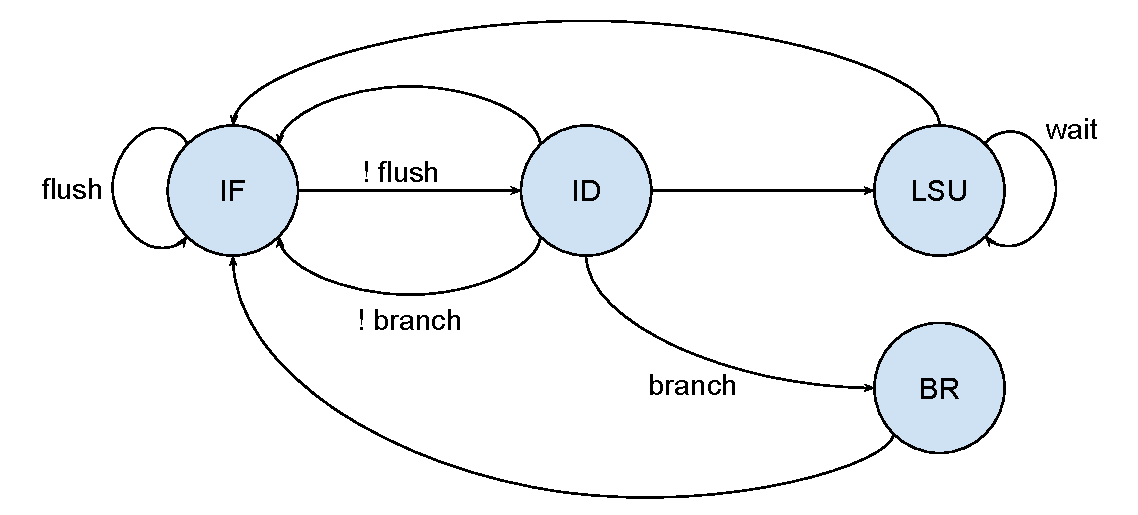
\includegraphics[width=\textwidth]{images/ri5cy-ppa.pdf}
	\caption{PPA extracted from the SystemC-PPA of the RI5CY core.}
	\label{fig:ri5cy-ppa}
\end{figure}

The important states depicted on the PPA correspond to the stages of the RI5CY pipeline. Even though the processor has a 4-stage pipeline, the register file was implemented as an external module, so there is no important state corresponding to this stage. Consequently, the behaviour of the signals that write to the register file is covered by the model and, therefore, by the generated property set. However, the register file functionality is not covered, and, as an independent module, it must have its own design and verification flow.

To illustrate the operations in the PPA of Fig.~\ref{fig:ri5cy-ppa}, consider an \textit{ADD} operation. It starts at the \textit{IF} state, and the first operation, represented by the edge from \textit{IF} to \textit{ID}, refers to when the instruction moves from the fetch stage to the decoder. The instruction fetching address is updated and a new request to the instruction memory is sent. The next operation starts in state \textit{ID}. In this operation, the add computation is done, and write back signals are set with the result and destination register address. Since all these steps happen in the same \textit{clock} cycle, they are part of the same operation. In addition, because the functionality of the register file is not part of the model, checking the correct write back signals is enough. Thus, there is no check on whether the right values are written to the registers or not. This behaviour would be covered by a separated property set for the register file module. Therefore, the ending state for this operation is already the \textit{IF} state as the execution of the instruction is done. The properties in the listing of Fig.~\ref{fig:ri5cy-if-id-micro-ppt-a} (a) and (b) show the two micro properties generated by \textit{DeSCAM} for the those two operations from \textit{IF} to \textit{ID} and from \textit{ID} back to \textit{IF}.

\begin{figure}[htb]
    \begin{lstlisting}
    property IF;
    dependencies: no_reset;
    for timepoints:
        t_end = t+1;
    freeze:
        iaddr_at_t = iaddr@t,
        [...]
    assume:
        at t: IF;
        at t: !(flush_in_sig);
        at t: !((getEncType(instr_in_sig) == enc_j));
        at t: !((getEncType(instr_in_sig) == enc_i_j));
    prove:
        at t_end: ID;
        at t_end: encodedInstr == instr_in_sig_at_t;
        at t_end: iaddr == (4 + iaddr_at_t)[31:0];
        at t_end: instr_req_sig == (4 + iaddr_at_t)[31:0];
        at t_end: pcIf == pcIf_at_t;
        at t_end: prevInstr == prevInstr_at_t;
        during[t+1, t_end]: data_out_notify == false;
        during[t+1, t_end-1]: instr_req_notify == false;
        at t_end: instr_req_notify == true;
        during[t+1, t_end]: toRegsPort_notify == false;
    end property;\end{lstlisting}
    \caption{(a) Micro property describing operation from \textit{IF} stage to \textit{ID} stage of RI5CY PPA}
    \label{fig:ri5cy-if-id-micro-ppt-a}
\end{figure}

\begin{figure}[htb]
\ContinuedFloat
    \begin{lstlisting}
    property ID;
    dependencies: no_reset;
    for timepoints:
    t_end = t+1;
    freeze:
        encodedInstr_at_t = encodedInstr@t,
        [...]
    assume:
        at t: ID;
        at t: !((getInstrType(encodedInstr) == instr_unknown));
        at t: (getEncType(encodedInstr) == enc_r);
    prove:
        at t_end: IF;
        at t_end: encodedInstr == encodedInstr_at_t;
        at t_end: iaddr == iaddr_at_t;
        at t_end: pcIf == iaddr_at_t;
        at t_end: prevInstr == prevInstr_at_t;
        at t_end: toRegsPort_sig_dst == getRdAddr(encodedInstr_at_t);
        at t_end: toRegsPort_sig_dstData == getALUres(getALUfunc(readRegfile(fromRegsPort_sig_reg_file_01_at_t,...),getRs1Addr(),getRs2Addr());
        during[t+1, t_end]: data_out_notify == false;
        during[t+1, t_end]: instr_req_notify == false;
        during[t+1, t_end-1]: toRegsPort_notify == false;
        at t_end: toRegsPort_notify == true;
    end property;\end{lstlisting}
    \caption{(b) Micro property describing operation from \textit{ID} stage to \textit{IF} stage of RI5CY PPA}
    \label{fig:ri5cy-if-id-micro-ppt-b}
\end{figure}

For simplicity, all the instructions comprised by the \textit{ENC\_R}, \textit{ENC\_I\_I}, \textit{ENC\_U}, \textit{ENC\_J}, and \textit{ENC\_I\_J} types have their operations represented by the \textit{IF-ID} and \textit{ID-IF} edges of the PPA in Fig.~\ref{fig:ri5cy-ppa}, although the properties generated for them are not the same. The \textit{load} and \textit{store} instructions for \textit{ENC\_I\_L} and \textit{ENC\_S} are represented by the four edges between states \textit{IF}, \textit{ID} and \textit{LSU}, including the wait edge. The \textit{branch} instructions of \textit{ENC\_B} are represented by two paths. One includes the \textit{branch} edge and comprises the three operations between the states \textit{IF}, \textit{ID} and \textit{BR}. This path corresponds to the execution when a branch is taken. The second path includes the \textit{!branch} edge that corresponds to the operation for when a branch is not taken. In this case, the branch instruction has only two operations between the states \textit{IF} and \textit{ID}. Finally, the \textit{flush} edge represents the operation when the pipeline is flushed. The \textit{!flush} edge is the regular operation between \textit{IF} and \textit{ID} for all instructions.

Running the Pipeline Algorithm for the property set generated by \textit{DeSCAM} will merge the micro and \textit{wait} operations resulting in pipeline properties. The micro properties in Fig.~\ref{fig:ri5cy-if-id-micro-ppt-a} (a) and (b) will be merged into a single property describing the behaviour through all pipeline stages. This is shown in the listing of Fig.~\ref{fig:ri5cy-enc-r-ppt}.

\begin{figure}[htb!]
    \begin{lstlisting}
    property ENC_R;
    dependencies: 
        no_reset,
        in_out_constraints,
        no_unaligned_case,
        no_hwlp_case,
        instr_mem;
    for timepoints:
        t_id = t+1,
        t_ex = t_id+1;
    freeze:
        iaddr_at_t = iaddr@t,
        instr_in_sig_at_t = instr_in_sig@t,
        encodedInstr_at_t_id = encodedInstr@t_id,
        fromRegsPort_sig_reg_file_01_at_t = fromRegsPort_sig_reg_file_01@t_id,
        [...] //remaining register variables
        iaddr_at_t_id = iaddr@t_id;
    assume:
        at t: IF;
        at t: !(flush_in_sig);
        at t: !((getEncType(instr_in_sig) == enc_j));
        at t: !((getEncType(instr_in_sig) == enc_i_j));
        
        at t_id: !((getInstrType(encodedInstr) == instr_unknown));
        at t_id: (getEncType(encodedInstr) == enc_r);
    prove:
        at t_id: encodedInstr == instr_in_sig_at_t;
        at t_id: iaddr == (4 + iaddr_at_t)[31:0];
        at t_id: instr_req_sig == (4 + iaddr_at_t)[31:0];
        during[t+1, t_id]: data_out_notify == false;
        at t_id: instr_req_notify == true;
        during[t+1, t_id]: toRegsPort_notify == false;
        
        at t_ex: pcIf == iaddr_at_t_id;
        at t_ex: toRegsPort_sig_dst == getRdAddr(encodedInstr_at_t_id);
        at t_ex: toRegsPort_sig_dstData == getALUresult(getALUfunc(encodedInstr_at_t_id, readRegfile(fromRegsPort_sig_reg_file_01_at_t,getRs1Addr(),getRs2Addr()));
        during[t_id+1, t_ex]: data_out_notify == false;
        at t_ex: toRegsPort_notify == true;
    end property;\end{lstlisting}
    \caption{Pipeline property for \textit{ENC\_R} instructions of RI5CY. This property is derived by merging the mirco properties in Fig.~\ref{fig:ri5cy-if-id-micro-ppt-a} (a) and (b).}
    \label{fig:ri5cy-enc-r-ppt}
\end{figure}

The property shown in Fig.~\ref{fig:ri5cy-enc-r-ppt} had some of its “\textit{freeze}” variables and function arguments omitted for simplicity reasons. The complete Pipeline Properties set can be found in \cite{descam}. The dependencies from lines 3 to 7 are the constraints valid for this property. The \textit{no\_reset} constraint is automatically added by \textit{DeSCAM} and corresponds to a macro which defines that there is no incoming reset signal during the instruction execution. The \textit{instr\_mem} constraint refines the instruction memory protocol. The three other constraints disable RI5CY extension modules, such as the non-aligned memory access and \textit{hardware loop} extensions. In this case study, only the RISC-V 32 bits base instruction is modelled. The \textit{in\_out\_constraints} constrains some unused \textit{inputs} and \textit{outputs}, such as interruption signals, to be de-asserted. 

The two timepoints were added and updated according to the two micro properties from which the pipeline property was merged. The $t\_id$ timepoint corresponds to the commitments of the micro property in Fig.~\ref{fig:ri5cy-if-id-micro-ppt-a}a, and $t\_ex$ for the commitments in Fig.~\ref{fig:ri5cy-if-id-micro-ppt-b}b. In addition, the “\textit{freeze}” variables from lines 12 to 17 had also their names updated according to the corresponding micro property timepoint.

The assumptions from line 19 to 22 correspond to the assumptions in Fig.~\ref{fig:ri5cy-if-id-micro-ppt-a}a. The \textit{IF} macro state is refined to represent both \textit{ready to fetch} and \textit{empty pipeline} states. The other three assumptions determine that there should be no flushing and that the fetched instruction is not a \textit{jump}, what would change the processor behaviour already at $t\_id$. The assumptions in lines 24 and 25 are imported from Fig.~\ref{fig:ri5cy-if-id-micro-ppt-b}b. They specify that the instruction to be decoded is known and of the type \textit{ENC\_R}. This determines the processor behaviour at $t\_ex$.

The commitments from lines 27 to 32 correspond to the operation \textit{IF-ID} from Fig.~\ref{fig:ri5cy-if-id-micro-ppt-a}a. As for the commitments from lines 34 to 38, they correspond to the operation \textit{ID-IF} from Fig.~\ref{fig:ri5cy-if-id-micro-ppt-b}b. By comparing the commitments of the micro properties and the merged property, it is possible to spot the inserted, deleted, and updated commitments by the merging steps of the pipeline algorithm. The helping macro functions are derived form the functions implemented in the ESL model, and they are fully automatically generated by \textit{DeSCAM}, so no refinement is needed. The remaining signals and state macros are generated in a separate file and must be refined by the designer to match the signals and registers of the RTL implantation. 

In addition to the properties for all the instruction types, a micro property for the \textit{flush} edge describing the behaviour of the flushing operation is generated by \textit{DeSCAM}, and it is refined by the Pipeline Algorithm. A property is also generated and refined for the operation when an unknown instruction is fetched. The assumptions for such property is shown in Fig.~\ref{fig:ri5cy-unknown-ppt}. An extra assumption, that is not part of the merging algorithm, is manually inserted, the \textit{illegal\_instr()} assumption. This assumption is only necessary in this special case study because not all instruction known to the RTL implementation are known to the ESL model. As a result, without this assumption, the property check tool would find a \textit{spurious} counter example with an instruction that is known to the RTL design, but not to the ESL model. In this case, the commitments would not be fulfilled, and the property would not hold. 

\begin{figure}[htb!]
    \begin{lstlisting}
    property UNKNOWN;
    [...]
    assume:
        at t: IF;
        at t: !(flush_in_sig);
        at t: !((getEncType(instr_in_sig) == enc_j));
        at t: !((getEncType(instr_in_sig) == enc_i_j));
        
        at t_id: (getInstrType(encodedInstr) == instr_unknown);
        //Manually added to exclude not covered instructions by ESL
        at t_id: illegal_instr (encodedInstr);
    prove:
    [...]
    end property;\end{lstlisting}
    \caption{Assumptions of the Pipeline Property that describes when a \textit{unknown} instruction is fetched.}
    \label{fig:ri5cy-unknown-ppt}
\end{figure}

Finally, a property with the assumptions such the ones shown in Fig.~\ref{fig:ri5cy-vacuous-ppt} is generated. This property assumes that the instruction fetched is not unknown but also not any of the known types. This results in an unreachable state. Therefore, the property checking tool classifies this property as a \textit{vacuous} pass, since no counter example nor witness can be found. In this context, witness means a valid example that is generated by the tool for which the property holds. 

\begin{figure}[htb!]
    \begin{lstlisting}
    property VACUOUS;
    [...]
    assume:
        at t: IF;
        at t: !(flush_in_sig);
        at t: !((getEncType(instr_in_sig) == enc_j));
        at t: !((getEncType(instr_in_sig) == enc_i_j));
        
        at t_id: !((getInstrType(encodedInstr) == instr_unknown));
        at t_id: !((getEncType(encodedInstr) == enc_r));
        at t_id: !((getEncType(encodedInstr) == enc_i_i));
        at t_id: !((getEncType(encodedInstr) == enc_i_l));
        at t_id: !((getEncType(encodedInstr) == enc_s));
        at t_id: !((getEncType(encodedInstr) == enc_b));
        at t_id: !((getEncType(encodedInstr) == enc_u));
        at t_id: !((getEncType(encodedInstr) == enc_j));
        at t_id: !((getEncType(encodedInstr) == enc_i_j));
    prove:
    [...]
    end property;\end{lstlisting}
    \caption{Assumptions of the Pipeline Property with an unreachable state where the fetched instruction is neither known nor unknown.}
    \label{fig:ri5cy-vacuous-ppt}
\end{figure}

\section{The \SSQED{} Properties}
\label{section:ri5cy-s2qed-ppt}

To make the set of pipeline properties complete, a set of \SSQED{} properties must be created. An overview about \SSQED{} can be seen in Sec.~\ref{section:s2qed}. The current section will present how a set of \SSQED{} properties was created to the RI5CY core.  Fig.~\ref{fig:ri5cy-enc-r-s2qed-ppt} shows a simplified \SSQED{} property for the instructions of type \textit{ENC\_R}. This example is going to be used to analyse each part of a \SSQED{} property.

\begin{figure}[htb!]
    \begin{lstlisting}
    property S2QED_ENC_R;
    [...]
    for timepoints:
        t_if_i1 = t,
        t_id_i1 = t_if_i1+1,
        t_wb_i1 = t_id_i1+1,
        t_done_i1 = t_wb_i1+1,
        
        t_if_i2 = t,
        t_id_i2 = t_if_i2+1..5 waits_for (CPU2_STALL == 0 && cpu2/id_ready == 1),
        t_wb_i2 = t_id_i2+1,
        t_done_i2 = t_wb_i2+1;
        [...]
    assume:
        // constraints on CPU1
        at t_if_i1: start_state && empty_pipeline;
        during [t_if_i1 + 1, t_done_i1]: cpu1/instr_rdata_i == 32'h13;
        // same instruction for IUV
        at t: !(getInstrType(cpu1/instr_rdata_i) == instr_unknown); 
        at t: getEncType(cpu1/instr_rdata_i) == enc_r;
        at t: cpu1/instr_rdata_i == cpu2/instr_rdata_i;
        at t: cpu1/instr_addr_o == cpu2/instr_addr_o;
        // QED consistent registers
        at t_wb_i2: foreach r in 0..31: 
        (regfile_i1_at_t_wb_i1[r] == REGISTER_CPU2(r) || (cpu2/regfile_we_wb && cpu2/regfile_waddr_fw_wb_o == resize(r,6))); 
        end foreach;
        at t_wb_i2: foreach r in 0..31: 
        (!cpu2/regfile_we_wb || cpu2/regfile_wdata == regfile_i1_at_t_wb_i1[r]); 
        end foreach;
        //Flushing
        during [t_if_i2, t_id_i2]: CPU2_NO_FLUSH_STATE;
        //I/O should be the same (no stalling)
        at t: CPU2_STALL == 0 && cpu2/id_ready == 1 && cpu2/if_stage_i/if_ready == 1;
    prove:
        // PC register
        at t_id_i2: cpu2/pc_if == cpu1_pcIf_at_t_id_1;
        // general registers
        at t_done_i2: cpu2/id_stage_i/registers_i/riscv_register_file_i/mem == regfile_i1_at_t_done_i1;
    end property;\end{lstlisting}
    \caption{\SSQED{} property for instructions of type \textit{ENC\_R}.}
    \label{fig:ri5cy-enc-r-s2qed-ppt}
\end{figure}

The \textit{dependencies} field was omitted because the constraints should follow the same construction idea as for the pipeline properties. For the timepoints, however, a major difference can be noticed; there are two set of time variables, one for each instance of the processor, \textit{cpu1} and \textit{cpu2}. Starting with \textit{cpu1}, the reader will notice that there are more timepoints than it would be expected if compared with the pipeline properties. This happens because the \SSQED{} focus on the consistency of the two CPU instances, rather than the result of the instruction operation. Consequently, checking the consistency between the register files demands an additional timepoint that relates to the time when the result is written back to the destination register. This additional timepoint corresponds to $t\_done$. Furthermore, the $t\_ex$ timepoint, which corresponds to the time when the ALU executes the operation and also when the write back signals are set, was renamed to $t\_wb$ to reflect the emphasis on the write back.

The assumptions start with the restrictions for \textit{cpu1}, stating that it is \textit{ready to fetch} at $t\_if$, it has an \textit{empty pipeline}, and that the instructions after the IUV are only \textit{nop}’s. This last assumption is not a requirement for the correctness of the model, instead it aims to reduce the complexity for the SAT-solving tool. Since the \SSQED{} properties have two independent instances executing, the complexity for the property checking tool and therefore the time needed for proving each property grows rapidly.

The next assumption refers to the IUV that must be of type \textit{ENC\_R}. Both CPU instances fetch the same instruction at $t\_if$. In addition, the \textit{output} address must also be the same. This assumption is important to be able to prove the consistency of the PC register. Next, the property assumes that the CPU instances are consistent at $t\_wb$. Finally, the last two assumptions refer to the \textit{cpu2} and requires that there is no flushing between $t\_if$ and $t\_id$, so that the IUV is not flushed, and that \textit{cpu2} is \textit{ready to fetch} at $t\_if$ when the IUV is fetched.

The two commitments are proving that the PC register of both CPU instances are consistent at $t\_id$, and that the register files are consistent at $t\_done$.

\subsection*{QED Consistency}

The base concept for QED consistency is presented in Sec.~\ref{section:s2qed} with emphasis on instructions of register type. However, the RTL implementation in this case study has an important particularity that requires further elaboration on consistency. The RI5CY core has two write back ports to the register file. One port for write back from the ALU, which is used for arithmetic and logic operations, and the other write back port is used by the LSU for loading data from the memory.

These two write back ports allow data to be written to two registers in the register file at the same time. Consider a scenario when there is a \textit{load} instruction followed by an \textit{add} instruction in \textit{cpu2}, and that the \textit{add} is the IUV. By the time the data is loaded from the memory, it is possible that the result from the \textit{add} operation is also available to write back. As a result, both loaded data from memory and add result will be written to their respective destination register at the same time. This would cause the \SSQED{} property to fail on the commitment of consistent register files at $t\_done$ because \textit{cpu1} will only write the add result from the ALU to its register file.

In order to deal with this simultaneous write back, the \textit{qed\_consistency\_registers} in Eq.~\ref{eq:consistency-register} in Sec.~\ref{section:s2qed} is modified to Eq.~\ref{eq:new-consistency-register}. $C$ and $U$ refer to the constrained \textit{cpu1} and unconstrained \textit{cpu2} respectively. $r^{t_{wb}}$ corresponds to the value of a specific register in the register file at $t\_wb$, $i^{t_{wb}}_r$ is the \textit{input} value to be written to register $r$ at $t\_wb$, and $w^{t_{wb}}_r $ is the write enable signal to register $r$ at $t\_wb$.

\begin{equation}
    qed\_consist\_reg := \bigwedge_{r \in U} \left((r^{t_{wb}}_U = r^{t_{wb}}_C) \lor w^{t_{wb}}_r\right) \land \bigwedge_{r \in U} \left(w^{t_{wb}}_r \rightarrow (i^{t_{wb}}_r = r^{t_{wb}}_C)\right)
    \label{eq:new-consistency-register}
\end{equation}

The extended qed\_consist\_reg of Eq.~\ref{eq:new-consistency-register} specifies that at $t\_wb$ either each register in \textit{cpu2} holds the same value as its corresponding register in \textit{cpu1}, or there is a write back for that register. If there is a write back to that register, the \textit{input} value to be written to the register is the same value that the corresponding register in \textit{cpu1} holds at $t\_wb$. This QED consistency is shown in lines 24 to 29 of the property in Fig.~\ref{fig:ri5cy-enc-r-s2qed-ppt}.

This QED consistency assumption of \textit{ENC\_R} instructions is also valid for the \textit{ENC\_U}, \textit{ENC\_J} and \textit{ENC\_I\_J}, as they use the same write back port from the ALU to write to the register file at $t\_wb$. The remaining instructions considered for this case study have the same previous QED consistency because they do not check the whole register file in the commitments at $t\_done$.

The \textit{load} instructions will check the consistency of the destination register after write back because the case of simultaneous access is covered by the properties for the instructions that uses the ALU write back port. The \textit{ENC\_S} instructions do not need to check the register files as they do not write to the registers. As shown in Fig.~\ref{fig:ri5cy-enc-s-s2qed-ppt}, it only checks PC and the consistency of the data memory output signals at $t\_ex$. The branch instructions will check the consistency of the PC register, \textit{branch decision} signal, and instruction fetching address for the case when the branch is taken, Fig.~\ref{fig:ri5cy-enc-b-s2qed-ppt-taken}, or simply the PC and \textit{branch signal} consistency for the case when the branch is not taken, Fig.~\ref{fig:ri5cy-enc-b-s2qed-ppt-not-taken}. The complete set of \SSQED{} properties is found in \cite{descam}.

\begin{figure}[htb!]
    \begin{lstlisting}
    property S2QED_ENC_S;
    [...]
    prove:
        // PC register
        at t_id_i2: cpu2/pc_if == cpu1_pcIf_at_t_id_1;
        
        // Data Memory Output
        at t_ex_i2: cpu2/data_req_o == data_req_at_ex_i1;
        at t_ex_i2: cpu2/data_we_o == data_we_at_ex_i1;
        at t_ex_i2: cpu2/data_addr_o == data_addr_at_ex_i1;
        at t_ex_i2: cpu2/data_wdata_o == data_wdata_at_ex_i1;
    end property;\end{lstlisting}
    \caption{Commitments of \SSQED{} property for \textit{ENC\_S} instructions.}
    \label{fig:ri5cy-enc-s-s2qed-ppt}
\end{figure}

\begin{figure}[htb!]
     \centering
     \begin{subfigure}[b]{\textwidth}
         \begin{lstlisting}
    property S2QED_ENC_B_TAKEN;
    [...]
    prove:
        // PC register
        at t_id_i2: cpu2/pc_if == cpu1_pcIf_at_t_id_1;
        at t_done_i2: cpu2/pc_if == cpu1_pcIf_at_t_done_1;
        
        // Branch Result
        at t_ex_i2: cpu2_flush_sig == cpu1_flush_sig_at_t_ex_i1;
        
        // Instr Memory Output
        at t_ex_i2: cpu2/instr_addr_o == instr_addr_at_t_ex_i1;
    end property;\end{lstlisting}
         \caption{Commitments of \SSQED{} property for \textit{ENC\_B} instructions when the branch is taken.}
         \label{fig:ri5cy-enc-b-s2qed-ppt-taken}
     \end{subfigure}
     \hfill
     \begin{subfigure}[b]{\textwidth}
         \begin{lstlisting}
    property S2QED_ENC_B_NOT_TAKEN;
    [...]
    prove:
        // PC register
        at t_id_i2: cpu2/pc_if == cpu1_pcIf_at_t_id_1;
        
        // Branch Result
        at t_ex_i2: cpu2_flush_sig == cpu1_flush_sig_at_t_ex_i1;
    end property;\end{lstlisting}
         \caption{Commitments of \SSQED{} property for \textit{ENC\_B} instructions when the branch is not taken.}
         \label{fig:ri5cy-enc-b-s2qed-ppt-not-taken}
     \end{subfigure}
        \caption{Commitments of \SSQED{} property for \textit{ENC\_B} instructions for both cases when the branch is (a) taken and (b) not taken.}
        \label{fig:ri5cy-enc-b-s2qed-ppt}
\end{figure}